\documentclass{beamer}
\usepackage[english, russian]{babel}
\usepackage[T2A]{fontenc}
\usepackage[utf8]{inputenc}
\usepackage{indentfirst}
\usepackage{amsmath, amsfonts, amssymb, amsthm, mathtools}
\usepackage[export]{adjustbox}
\usepackage{graphicx} 
\graphicspath{ {./images/} }

\usepackage{subcaption}
\usepackage{verbatim}

\usepackage{minted}{\setlength{\parskip}{0pt}}

\usepackage{hyperref}

\hypersetup{
    colorlinks=true,
    linkcolor=blue,
    filecolor=magenta,      
    urlcolor=black,
    pdftitle={Overleaf Example},
    pdfpagemode=FullScreen,
    }


\title{Отчет по лабораторной работе № 12. \\ Синхронизация времени}
\author{Данила Стариков \\ НПИбд-02-22}
\date{2024}

\begin{document}

\maketitle
\newpage

\tableofcontents

\newpage
\section{Цель работы}
Получение навыков по управлению системным временем и настройке синхронизации времени.

\newpage
\section{Выполнение работы}
\subsection{Настройка параметров времени}
\begin{enumerate}
\item На сервере и клиенте посмотрели параметры настройки даты и времени (Рис. \ref{01} и \ref{02}):
  \begin{minted}{bash}
    timedatectl
  \end{minted}
\begin{center}
    \centering
    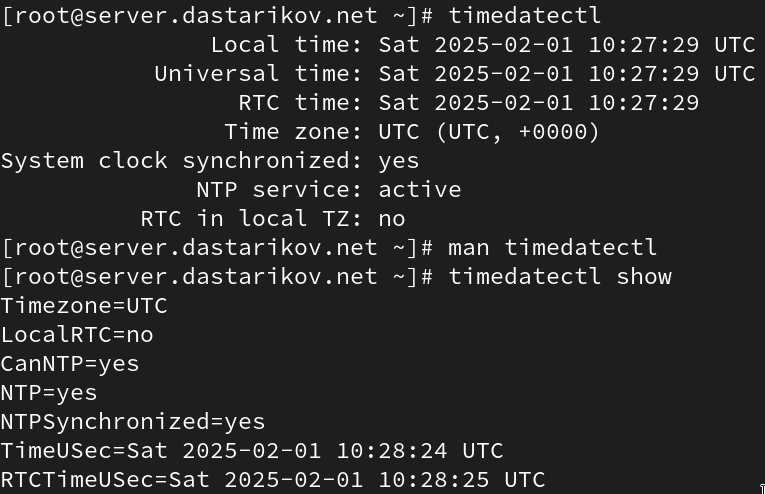
\includegraphics[width=\textwidth]{../images/image01.png}
    \captionof{figure}{Информация о дате и времени на сервере (timedatectl).}
    \label{01}
\end{center}
\begin{center}
    \centering
    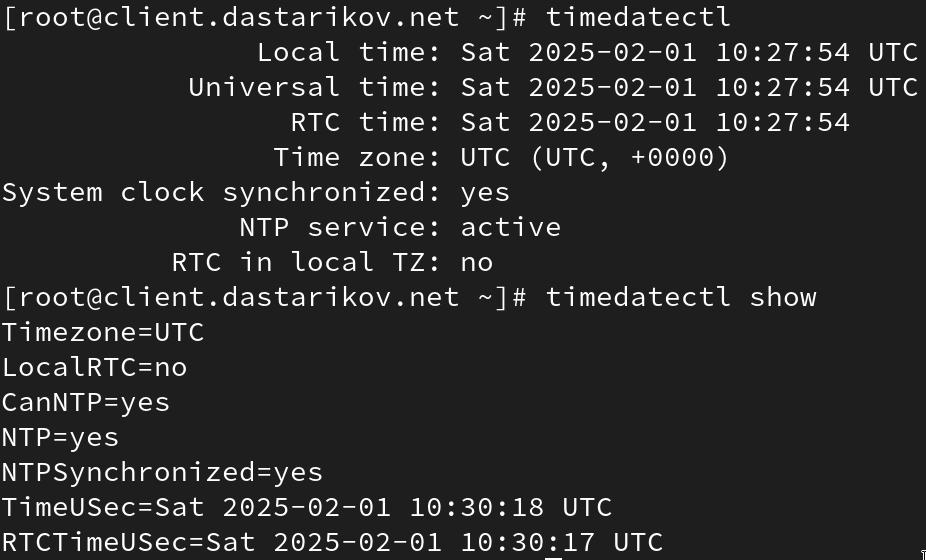
\includegraphics[width=\textwidth]{../images/image02.png}
    \captionof{figure}{Информация о дате и времени на клиенте (timedatectl).}
    \label{02}
\end{center}

  % Определите, в какой временной зоне находятся сервер и клиент, проводится ли сетевая синхронизация времени и т.п. Поэкспериментируйте с параметрами этой команды.
\item На сервере и клиенте посмотрели текущее системное время (Рис. \ref{04} и \ref{03}):
  \begin{minted}{bash}
    date
  \end{minted}
\begin{center}
    \centering
    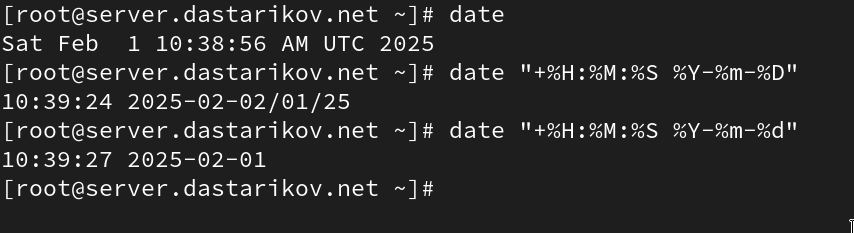
\includegraphics[width=\textwidth]{../images/image04.png}
    \captionof{figure}{Вывод команды \texttt{date} с разными ключами на сервере.}
    \label{04}
\end{center}
\begin{center}
    \centering
    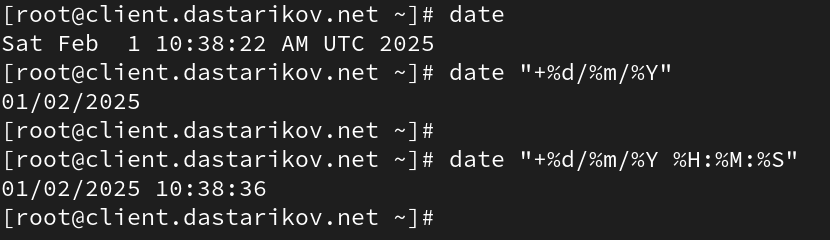
\includegraphics[width=\textwidth]{../images/image03.png}
    \captionof{figure}{Вывод команды \texttt{date} с разными ключами на клиенте.}
    \label{03}
\end{center}

%  Поэкспериментируйте с параметрами этой команды.
\item На сервере и клиенте посмотрели аппаратное время (Рис. \ref{07} и \ref{06}):
  \begin{minted}{bash}
    hwclock
  \end{minted}
\begin{center}
    \centering
    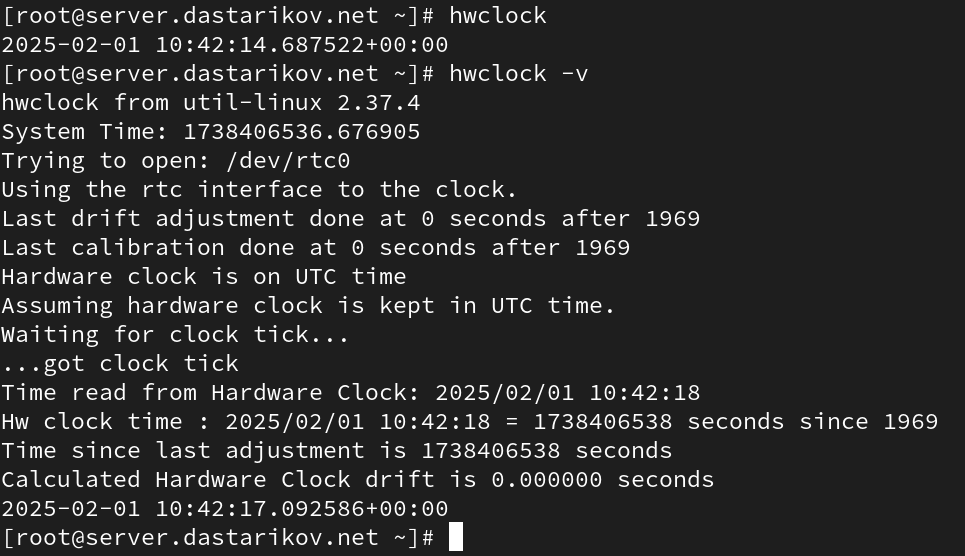
\includegraphics[width=\textwidth]{../images/image07.png}
    \captionof{figure}{Вывод команды \texttt{hwclock} с разными ключами на сервере.}
    \label{07}
\end{center}
\begin{center}
    \centering
    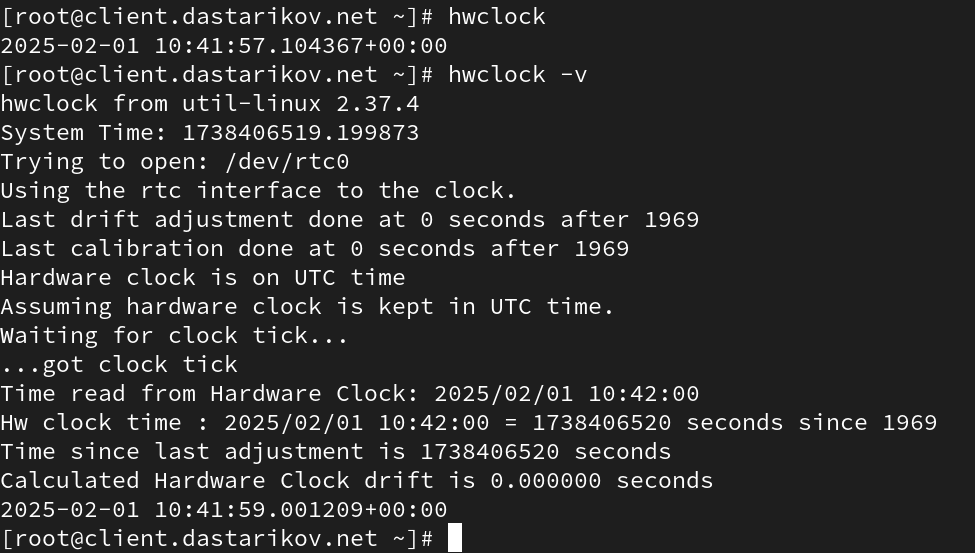
\includegraphics[width=\textwidth]{../images/image06.png}
    \captionof{figure}{Вывод команды \texttt{hwclock} с разными ключами на клиенте.}
    \label{06}
\end{center}
\end{enumerate}
\subsection{Управление синхронизацией времени}
\begin{enumerate}
\item При необходимости установили на сервере необходимое программное обеспечение:
  \begin{minted}{bash}
    dnf -y install chrony
  \end{minted}
\item Проверили источники времени на клиенте и на сервере (Рис. \ref{08} и \ref{09}):
  \begin{minted}{bash}
    chronyc sources
  \end{minted}
\begin{center}
    \centering
    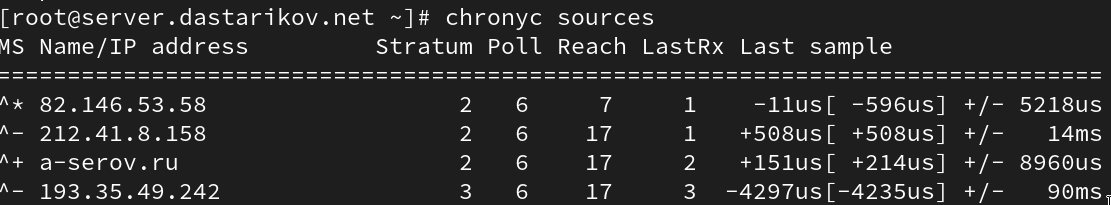
\includegraphics[width=\textwidth]{../images/image08.png}
    \captionof{figure}{Проверка источников времени на сервере.}
    \label{08}
\end{center}
\begin{center}
    \centering
    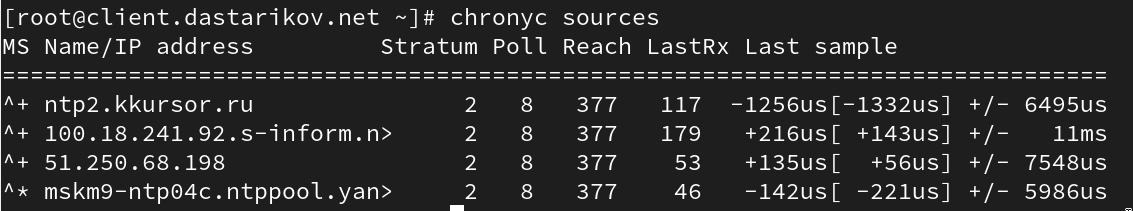
\includegraphics[width=\textwidth]{../images/image09.png}
    \captionof{figure}{Проверка источников времени на клиенте.}
    \label{09}
\end{center}

%  В отчёте поясните выведенную информацию.
\item На сервере открыли на редактирование файл \texttt{/etc/chrony.conf} и добавили строку:
  \begin{minted}{bash}
    allow 192.168.0.0/16
  \end{minted}
\item На сервере перезапустили службу \texttt{chronyd} (Рис. \ref{11}):
  \begin{minted}{bash}
    systemctl restart chronyd
  \end{minted}
\item Настроили межсетевой экран на сервере (Рис. \ref{11}):
  \begin{minted}{bash}
    firewall-cmd --add-service=ntp --permanent
    firewall-cmd --reload
  \end{minted}
\begin{center}
    \centering
    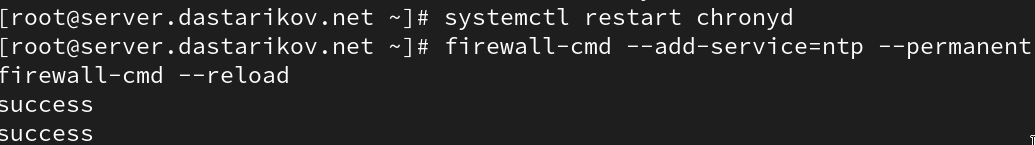
\includegraphics[width=\textwidth]{../images/image11.png}
    \captionof{figure}{Перезапуск \texttt{chronyd} и настройка межсетевого экрана.}
    \label{11}
\end{center}

\item На клиенте откроили файл \texttt{/etc/chrony.conf} и добавили строку (Рис. \ref{12}):
  \begin{minted}{bash}
    server server.dastarikov.net iburst
  \end{minted}
\begin{center}
    \centering
    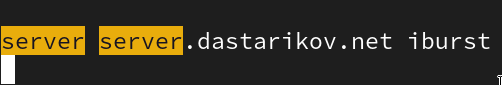
\includegraphics[width=\textwidth]{../images/image12.png}
    \captionof{figure}{Изменение файла конфигурации \texttt{chrony}.}
    \label{12}
\end{center}

  Удалили все остальные строки с директивой \texttt{server}.
\item На клиенте перезапустили службу \texttt{chronyd}:
  \begin{minted}{bash}
    systemctl restart chronyd
  \end{minted}

\item Проверили источники времени на клиенте и на сервере (Рис. \ref{14} и \ref{15}):
  \begin{minted}{bash}
    chronyc sources
  \end{minted}
\begin{center}
    \centering
    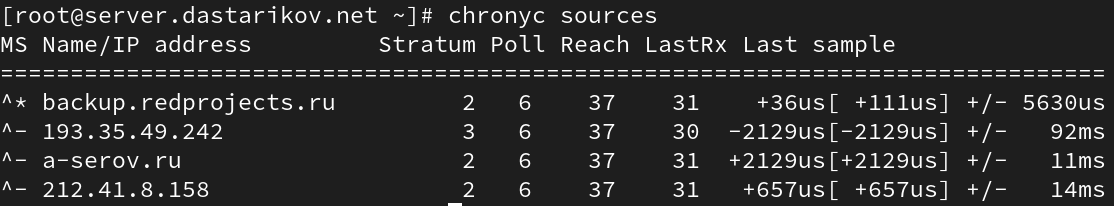
\includegraphics[width=\textwidth]{../images/image14.png}
    \captionof{figure}{Просмотр источников времени на сервере.}
    \label{14}
\end{center}

\begin{center}
    \centering
    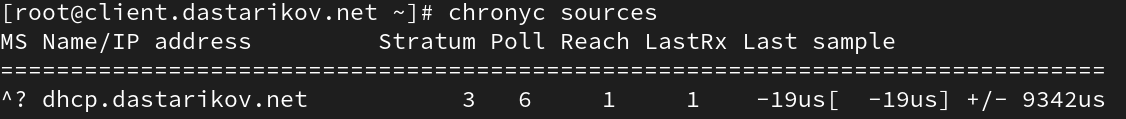
\includegraphics[width=\textwidth]{../images/image15.png}
    \captionof{figure}{Проверка добавленного источника времени на клиенте.}
    \label{15}
\end{center}

%  В отчёте поясните выведенную информацию.
% \item Посмотрели подробную информацию о синхронизации и пояснили в отчёте выведенную на экран информацию.
\end{enumerate}

\subsection{Внесение изменений в настройки внутреннего окружения виртуальных машин}
\begin{enumerate}
\item На виртуальной машине \texttt{server} перешли в каталог для внесения изменений в настройки внутреннего окружения \texttt{/vagrant/provision/server/}, создали в нём каталог \texttt{ntp}, в который поместили в соответствующие подкаталоги конфигурационные файлы (Рис. \ref{16}):
  \begin{minted}{bash}
    cd /vagrant/provision/server
    mkdir -p /vagrant/provision/server/ntp/etc
    cp -R /etc/chrony.conf /vagrant/provision/server/ntp/etc/
  \end{minted}
\item В каталоге \texttt{/vagrant/provision/server} создали исполняемый файл \texttt{ntp.sh} (Рис. \ref{16}):
  \begin{minted}{bash}
    cd /vagrant/provision/server
    touch ntp.sh
    chmod +x ntp.sh
  \end{minted}
\begin{center}
    \centering
    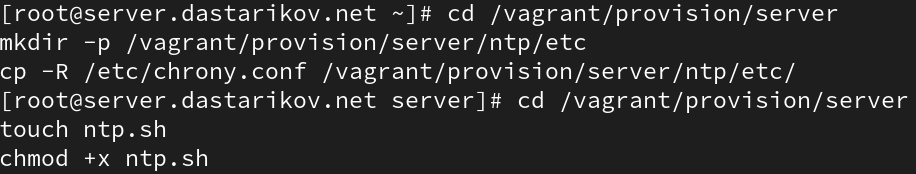
\includegraphics[width=\textwidth]{../images/image16.png}
    \captionof{figure}{Настройка внутреннего окружения виртуальной машины сервера.}
    \label{16}
\end{center}

  Открыв его на редактирование, прописали в нём следующий скрипт:
  \begin{minted}{bash}
    #!/bin/bash
    echo "Provisioning script $0"
    echo "Install needed packages"
    dnf -y install chrony
    echo "Copy configuration files"
    cp -R /vagrant/provision/server/ntp/etc/* /etc
    restorecon -vR /etc
    echo "Configure firewall"
    firewall-cmd --add-service=ntp
    firewall-cmd --add-service=ntp --permanent
    echo "Restart chronyd service"
    systemctl restart chronyd
  \end{minted}
\item На виртуальной машине \texttt{client} перешли в каталог для внесения изменений в настройки внутреннего окружения \texttt{/vagrant/provision/client/}, создали в нём каталог \texttt{ntp}, в который поместили в соответствующие подкаталоги конфигурационные файлы (Рис. \ref{18}):
  \begin{minted}{bash}
    cd /vagrant/provision/client
    mkdir -p /vagrant/provision/client/ntp/etc
    cp -R /etc/chrony.conf /vagrant/provision/client/ntp/etc/
  \end{minted}
\item В каталоге \texttt{/vagrant/provision/client} создали исполняемый файл \texttt{ntp.sh} (Рис. \ref{18}):
  \begin{minted}{bash}
    cd /vagrant/provision/client
    touch ntp.sh
    chmod +x ntp.sh
  \end{minted}
\begin{center}
    \centering
    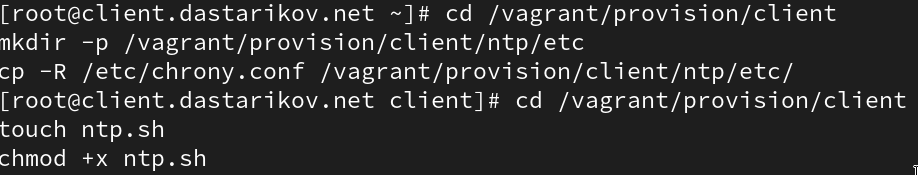
\includegraphics[width=\textwidth]{../images/image18.png}
    \captionof{figure}{Настройка внутреннего окружения виртуальной машины клиента.}
    \label{18}
\end{center}
  Открыв его на редактирование, прописали в нём следующий скрипт:
  \begin{minted}{bash}
    #!/bin/bash
    echo "Provisioning script $0"
    echo "Copy configuration files"
    cp -R /vagrant/provision/client/ntp/etc/* /etc
    restorecon -vR /etc
    echo "Restart chronyd service"
    systemctl restart chronyd
  \end{minted}
\item Для отработки созданных скриптов во время загрузки виртуальных машин \texttt{server} и \texttt{client} в конфигурационном файле Vagrantfile добавили в соответствующих разделах конфигураций для сервера и клиента:
  \begin{minted}{bash}
    server.vm.provision "server ntp",
    type: "shell",
    preserve_order: true,
    path: "provision/server/ntp.sh"
    client.vm.provision "client ntp",
    type: "shell",
    preserve_order: true,
    path: "provision/client/ntp.sh"
  \end{minted}
\end{enumerate}

\section{Выводы}
В результате выполнения лабораторной работы получили навыки по управлению системным временем и настройке синхронизации времени.
\end{document}
